\documentclass{beamer}

% For more themes, color themes and font themes, see:
% http://deic.uab.es/~iblanes/beamer_gallery/index_by_theme.html
%
\mode<presentation>
{
  \usetheme{default}       % or try default, Darmstadt, Warsaw, ...
  \usecolortheme{beaver} % or try albatross, beaver, crane, ...
  \usefonttheme{serif}    % or try default, structurebold, ...
  \setbeamertemplate{navigation symbols}{}
  \setbeamertemplate{caption}[numbered]
} 

\usepackage[german]{babel}
\usepackage[utf8x]{inputenc}
\usepackage{chemfig}
\usepackage[version=3]{mhchem}
\usepackage{listings}
\usepackage{graphicx}

% On Overleaf, these lines give you sharper preview images.
% You might want to `comment them out before you export, though.
\usepackage{pgfpages}
\pgfpagesuselayout{resize to}[%
  physical paper width=8in, physical paper height=6in]

% Here's where the presentation starts, with the info for the title slide
\title{Schema.org Injector}
\titlegraphic{
\includegraphics[width=.25\textwidth,height=.25\textheight]{icon.png}}
\subtitle{Final presentation}
\author{Stefan Haberl, Mathias Meinschad}
\institute{STI Innsbruck}
\date{February 3, 2017}

\begin{document}

% % % % % % % % % % % % %
% TITLE PAGE
% % % % % % % % % % % % %
\begin{frame}
  \titlepage
\end{frame}

% % % % % % % % % % % % %
% OVERVIEW
% % % % % % % % % % % % %
\begin{frame}{Overview}
  \tableofcontents
\end{frame}

% % % % % % % % % % % % %
% PROJECT
% % % % % % % % % % % % %
\section{Project}
\begin{frame}{Project}
	Developing an extension for the CMS-system \textcolor{blue}{\textbf{TYPO3}}, which allows the users to inject schema.org annotations inside their webpages.
	Each page can be associated with JSON-LD files, which then are injected into the pages \textcolor{blue}{\textbf{head tag}}. 
	
	\begin{block}{Specification}
		\begin{itemize}
			\item Inject JSON-LD into single page
			\item Inject JSON-LD into multiple pages
			\item Easy to set up and intuitive customizations
			\item Compatibility to as many TYPO3 versions as possible
		\end{itemize}
	\end{block}
\end{frame}

\begin{frame}[fragile]
\frametitle{JSON-LD}
\begin{block}{}
	\begin{lstlisting}
		<script type="application/ld+json">
		{
		  "@context": "http://schema.org/",
		  "@type": "Person",
		  "name": "Albert Einstein"
		}
		</script>
	\end{lstlisting}
\end{block}

\begin{block}{Why JSON-LD?}
	\begin{itemize}
	\item easy readable for humans and machines
	\item standard libraries for nearly any programming language
	\item difference between JSON and JSON-LD: extending known format with additional keys (e.g. context)
	\end{itemize}
\end{block}

\end{frame}

\begin{frame}{Typo3 CMS}
	\begin{block}{Overview}
		\begin{itemize}
			\item Typo3 is an open source Content Managment System
			\item developed by: Kasper Skårhøj
			\item released: 1998
			\item current version: 8.5.1 (January 25, 2017)
			\item languages: PHP, SQL und JavaScript
			\item Building page with TypoScript and Fluid
		\end{itemize}
	\end{block}
	
	\begin{block}{What is a Content Managment System (CMS)?}
		CMS is a software for handling (create, update, delete) contents inside a webpage.
	\end{block}

\end{frame}

% % % % % % % % % % % % %
% OUR EXTENSION
% % % % % % % % % % % % %
\section{Our Extension and how it works}
\begin{frame}{Our Extension}
	\begin{block}{General}
		\begin{itemize}
			\item TYPO3 uses extension keys to allow unique identifying each extension
			\item extension key registered:  \textbf{schema\textunderscore injector}
			\item Developed with JetBrains PhpStorm
			\item XAMPP for local testing
			\item Will be published in TEM (Typo3 Extension Repository)
		\end{itemize}
	\end{block}
	
	\begin{block}{Technical}
		\begin{itemize}
			\item using hooks to manipulated rendered data
			\item persist settings into database
			\item use page ID to check if an injection is configured for a specific page
		\end{itemize}
	\end{block}
\end{frame}

\begin{frame}{How it works}
	\begin{figure}[ht]
		\centering
		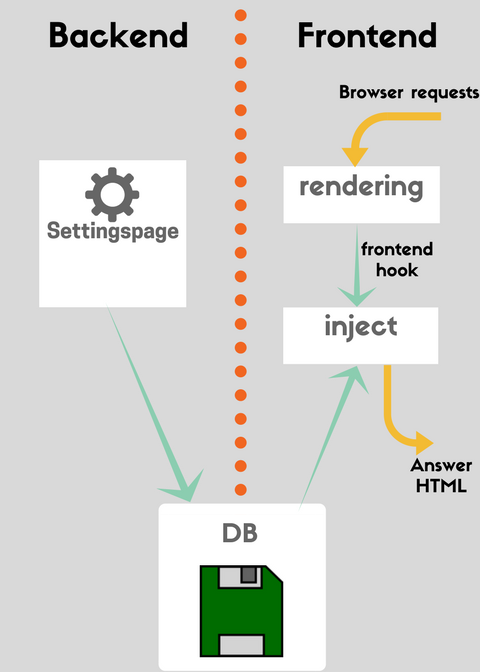
\includegraphics[height=0.75\textwidth]{work_flow.png}
	\end{figure}
\end{frame}

% % % % % % % % % % % % %
% LIVE DEMO
% % % % % % % % % % % % %
\section{Live Demo}
\begin{frame}{Live Demo}
	\begin{figure}[ht]
		\centering
		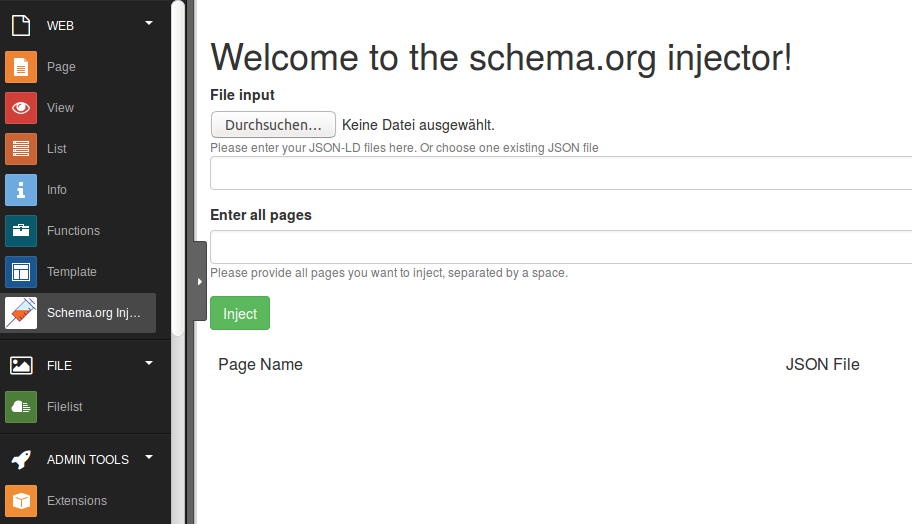
\includegraphics[width=1.0\textwidth]{backend_module.png}
	\end{figure}
\end{frame}

% % % % % % % % % % % % %
% OUR PROBLEMS
% % % % % % % % % % % % %
\section{Our Problems}
\begin{frame}{Our Problems}
	\begin{itemize}
		\item No experience with Typo3
		\item Caching behaviour in Typo3 while development (can't be completely turned off)
		\item Documentation is often out of date
		\item Small community, nearly no forums
		\item Low basic knowledge in PHP
		\item Solutions for older version not suitable for us
		\item Typo3 in general: TypoScript, how to inject code \dots
	\end{itemize}
\end{frame}

% % % % % % % % % % % % %
% FURTHER STEPS
% % % % % % % % % % % % %
\section{Outcome}
\begin{frame}{Outcome}
	
	\begin{block}{What we stated before Christmas}
			\begin{itemize}
	\item \textcolor{green}{\textbf{Done}} Define the UI
	\item \textcolor{green}{\textbf{Done}} Develop the database entity for user settings
	\item \textcolor{green}{\textbf{Done}} Develop main functionality
	\item \textcolor{green}{\textbf{Done}} Test main functionality
	\item \textcolor{orange}{\textbf{In progress}} Documentation
	\end{itemize}
	\end{block}
	
	\begin{block}{What's next?}
		\begin{itemize}
			\item Publishing on TER (Typo3 Extension Repository)
			\item Finish documentation in Sphinx
		\end{itemize}
	\end{block}
\end{frame}

\begin{frame}{}
	ANY QUESTIONS?
\end{frame}

\begin{frame}{Thanks a lot!}
	Thank you for your attention!
\end{frame}

\end{document}